\section{Methods of signal reconstruction}
One of the most difficult challenges of operationg a KID is to convert the $I(t)$ and $Q(t)$ values to an absorbed optical power or shift in resonant frequency as a function of time $\delta f_{0} \propto \delta P_{opt}$. In this section, we will see how to adress this problem by using a new modulated readout technique and then by using two different signal reconstruction methods : RfdIdQ and Cf.

\subsection{Modulated readout technique}
An innovative readout technique has been developed to monitor the change of the signal $\frac{dI}{df}$,$\frac{dQ}{df}$ by using a known frequency shift. This scheme allows continuous simultaneous tracking of KID resonant frequency which change proportionally to the absorbed optical power. To do so, the standart excitation of the detectors which uses a fixed tone is replaced by a new excitation based on two different frequencies. In fact, in order to generate two tones, we modulate the local oscillator signal between two values, separated by $\delta f_{LO} \simeq 1$ kHz, and obtain $f_{+} = f_{0} + \frac{\delta f_{LO}}{2}$ and $f_{-} = f_{0} - \frac{\delta f_{LO}}{2}$ with $f_{0}$ the detector resonant frequency.\\
The values ($I(t)$,$Q(t)$) are then given by :

\begin{equation}
(I(t),Q(t)) = (\frac{I(f_{+}) + I(f_{-})}{2}, \frac{Q(f_{+}) + Q(f_{-})}{2})
\end{equation}

and the differential values are :

\begin{equation}
\label{gradient}
(\frac{dI}{df}(t),\frac{dQ}{df}(t)) = (\frac{I(f_{+}) - I(f_{-})}{\delta f_{LO}}, \frac{Q(f_{+}) - Q(f_{-})}{\delta f_{LO}})
\end{equation}

\begin{figure}[h]
\center
	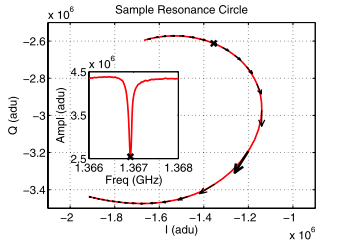
\includegraphics[scale=0.5]{resonance-circle.png}
	\caption{Representation in the I-Q plane of a sweep around a resonance. The red line represents the $(I,Q)$ data of the frequency sweep around the resonance.The arrows reprsents ($\frac{dI}{df}$,$\frac{dQ}{df}$). \citep{2013A&A...551L..12C}}
	\label{circle-iq}
\end{figure}

Fig. \ref{circle-iq} shows a typical KID resonance circle. Thanks to this modulation technique, we obtain four quantities : I, Q and their variation $\delta I$, $\delta Q$.\\
In this paper, I(t) and Q(t) are sampled at 22 Hz, they are the mean values of sub-sample i(t) and q(t) on $N_{m}$ = 40 points at 880 Hz. dI(t) and dQ(t) are the mean values of the difference between the data measured at $f_{-}$ and $f_{+}$. Then we have :

\begin{equation}
I = \sum^{N_{m}=40}_{p=1} i_{p}
\end{equation}

\begin{equation}
Q = \sum^{N_{m}=40}_{p=1} q_{p}
\end{equation}

\begin{equation}
dI = \sum^{N_{m}/2=20}_{p=1} i_{2p} - i_{2p-1}
\end{equation}

\begin{equation}
dQ = \sum^{N_{m}/2=20}_{p=1} q_{2p} - q_{2p-1}
\end{equation}

As shown in the next paragraph, these quantities are used to reconstruct the resonance frequency and so the optical power absorbed by the detector.

\subsection{RfdIdQ}
To reconstruct the signal absorbed by the detector, a method was developed named RfdIdQ.\\
If a variation $\Delta I(t)$, $\Delta Q(t)$ is observed between successive  ($I(t)$, $Q(t)$) points, it is possible to estimate the value of $\delta f_{0}$ by comparing ($\Delta I(t)$, $\Delta Q(t)$) with the gradient $(\frac{dI}{df}(t),\frac{dQ}{df}(t)) $. This is done by projecting ($\Delta I(t)$, $\Delta Q(t)$) along the gradient found in Eq.\ref{gradient}. The shift of the resonant frequency between two samples is then determined with Eq.\ref{Rf} \citep{2014A&A...569A...9C}

\begin{equation}
\label{Rf}
\Delta (\delta f_{0}(t)) = \delta f_{LO} \frac{\Delta I<dI>_{50} + \Delta Q<dQ>_{50} }{<dI>_{50}^{2} + <dQ>_{50}^{2}}
\end{equation}

\begin{equation}
\delta f_{0}(t) = \sum^{t}_{t'=0} (\Delta (\delta f_{0})(t'))
\end{equation}

\footnote{$<.>_{50}$ means that we average the considered quantities over 50 points before and after the concerned value.}

This method is convenient, but can be affected by some systematic uncertainty and be a source of non-linearity. In fact, $(\frac{dI}{df}(t),\frac{dQ}{df}(t))$ is tangeant to the (I,Q) circle for a fixed background optical power, whereas the actual variation ($\Delta I$, $\Delta Q$) (occurs for a fixed excitation frequency and is due to a difference in the optical power, which includes a change in the (I,Q) circle radius.). As a consequence, the observed (I,Q) trajectory is not precisely parallel to the direction given by $(\frac{dI}{df}(t),\frac{dQ}{df}(t))$. The predicted error induced by the projection method is less than 2\% for faint sources \citep{2013A&A...551L..12C}. In addition, by averaging $dI$ and $dQ$ we apply a $dI$,$dQ$ that can be very different from reality, in particular when we are near the resonance, with a bright source.\\

\subsection{Cf}
To compensate for the errors brought by the rfdidq method, we developed a new technique named Cf (circle fit).\\
The idea of this method is to project I, Q, dI, dQ, onto an axis $y_{3}$ which is as linear as possible with frequency, and so is assumed to be linear with the optical power. In fact, we suppose that :

\begin{equation}
\label{hyp-f}
f = f_{0} + \frac{w}{2} tan\frac{\phi}{2}
\end{equation}

We know that when near a resonance $Z = I+jQ$ is on a circle. To construct $y_{3}$ we scale, translate, rotate and inverse the initial circle to transform it into an infinite radius circle described by :

\begin{equation}
\label{Zres}
Z_{res} = 1 - i tan\frac{\varphi}{2}
\end{equation}

According to Eq. \ref{hyp-f}, the imaginary part of $Z_{res}$ is linearly dependant with the frequency and so represents $y_{3}$, $y_{3} \propto f - f_{0}$.\\
Here to calibrate this dependency and reconstruct the signal, we use I, Q, dI and dQ measurements. By applying the transformations, I, Q, dI and dQ become : 

\begin{equation}
I_{res} = - \frac{1}{2r}[(I-x_{c})cos\alpha + (Q - y_{c})sin \alpha] + \frac{1}{2}
\end{equation}
\begin{equation}
 Q_{res} = \frac{1}{2r}[-(I-x_{c})sin\alpha + (Q - y_{c})cos \alpha] 
\end{equation}

\begin{equation}
dI_{res} = -\frac{1}{2r}(dI cos\alpha + dQ sin\alpha)
\end{equation}

\begin{equation}
dQ_{res} = \frac{1}{2r}(-dI sin\alpha + dQ cos\alpha)
\end{equation}

with : ($x_{c}, y_{c}$), r and $\alpha$ respectively, the center, radius and rotation angle of the initial circle.\\
Then, $dy_{3} = Im(dZ_{res})$. According to the hypothesis in Eq. \ref{hyp-f}, f is a polynom, so to reconstruct the shift in the resonant frequency we can easily fit $\frac{\Delta f}{dy_{3}}$ by a polynomial function and integrate it to obtain the relative frequency of the KID.

%In the next section we describe an innovative modulated readout schemewhich enables the opti- cal power absorbed by a KID to be continuously monitored and leads to a large improvement in the consistency of the photomet- ric calibration.

\subsection{Simulations}
To adress the KIDs non-linearity, we need to measure its non-linearity coefficient $\varepsilon$ by doing simulations of the KID response to an incoming source of radiation, using the Rfdidq and Cf methods.

	\subsubsection{Method}
The simulation method consists first in modelling a scan of planet with a more or less important flux, at a certain speed. Then we recalculate the incoming flux thanks to the modulation technique and the rf/cf method. Finally, we stock the outcoming flux to be able to deduce the non-linearity coefficient.

	\subsubsection{Results}
graphe epsilon vs fwhm
